\documentclass[aps,pra,10pt,floatfix,nofootinbib]{revtex4-1}

\usepackage{bbm}
\usepackage{amsmath}
\usepackage{amssymb}
\usepackage{graphicx}
\usepackage{amsfonts}
\usepackage{amsthm}
\usepackage{tikz}

\newtheorem{thm}{Theorem}[section]
\newtheorem{cor}[thm]{Corollary}
\newtheorem{lem}[thm]{Lemma}
\newtheorem{prop}[thm]{Proposition}

\theoremstyle{definition}
\newtheorem{defn}[thm]{Definition}
\newtheorem*{assump1}{Classical assumption}
\newtheorem*{assump2}{Determinism and Reversibility assumption}

\begin{document}
	
\section{Classical mechanics in one post}

TL;DR Classical mechanics describes a divergence-free flow of states. The Hamiltonian is the time component of its vector potential. The Lagrangian is the scalar product between the flow and the vector potential.

For the longest time I didn't know what the Lagrangian was and why its integral is minimized along trajectories. A couple of months ago I went through Mathematical Methods of Classical Mechanics by V.I. Arnold and found some insights into differential geometry that got me going and finally worked out a satisfactory answer. I unpacked that understanding in a way that only needs differential calculus, so that it's more understandable and gives direct physics intuition. If you have studied magnetostatics (i.e. the magnetic field and its vector potential) you should be able to fully follow this.

\section{Deterministic and reversible flow}

Take the space formed by position $x$, momentum $p$ and time $t$. This is sometimes called the extended phase space: it represents all states at all times.

The evolution of a state in time is represented by a line in this space. If we have a law of evolution, at each point we have a vector that tells us where the state is going to move. This forms a vector field
\begin{equation}
\begin{aligned}
\vec{S} &= \dfrac{dx}{dt} e_x + \dfrac{dp}{dt} e_p + \dfrac{dt}{dt} e_t \\ 
&= S^x e_x + S^p e_p + S^t e_t 
\end{aligned}
\label{flow}
\end{equation}
 on the extended phase space, which we call flow. $e_x$, $e_p$ and $e_t$ are the unit vectors along each direction, which are multiplied by the respective components of $\vec{S}$.

Note that, since we are using time both as a coordinate and as the parametrization of the curve, the time component of $\vec{S}$ is unitary: $S^t = \dfrac{dt}{dt} = 1$. Also, we are going to assume that the surface integral of $\vec{S}$ on a closed curve is zero: the density of states that flows in is equal to the density of states that flows out. In this sense, I call this deterministic and reversible flow. Well, there are a dozen other reasons to call it that, but we will see them some other time.

If you remember your vector calculus, you know that we can define a vector potential for a divergence-free field. We therefore define
\begin{equation}
\begin{aligned}
\vec{\theta} &= p \, e_x + 0 \, e_p - H(x,p,t) \, e_t \\ 
&= \theta^x e_x + \theta^p e_p + \theta^t e_t 
\end{aligned}
\label{potential}
\end{equation}
This is actually the opposite of the vector potential: we need an annoying minus sign to match with existing conventions. We have
\begin{equation}
\begin{aligned}
\vec{S} &= \mathrm{curl}(-\vec{\theta}) = - \nabla \times \vec{\theta} \\
S^x &= \dfrac{dx}{dt} = - \partial_p \theta^t + \partial_t \theta^p = \partial_p H + \partial_t 0 = \partial_p H \\
S^p &= \dfrac{dp}{dt} = - \partial_t \theta^x + \partial_x \theta^t = -\partial_t p - \partial_x H = - \partial_x H \\
S^t &= \dfrac{dt}{dt} = - \partial_x \theta^p + \partial_p \theta^x = - \partial_x 0 + \partial_p p = 1
\end{aligned}
\label{HamiltonEquations}
\end{equation}

We recognize Hamilton's equations. Geometrically, the Hamiltonian is the time component of the vector potential while conjugate momentum is the spatial component.

\section{Line integral of the vector potential}

The line integral of a vector field $\vec{\theta}$ has an interesting, yet little known property: it is stationary along the field lines $\gamma$ of the curl. That is: if we make a small change in the line $\gamma$, the line integral $\int \vec{\theta} \cdot d\vec{\gamma}$ does not change. In other words:

\begin{equation}
\delta \int \vec{\theta} \cdot d\vec{\gamma} = 0
\label{stationaryLineIntegral}
\end{equation}

\begin{figure}
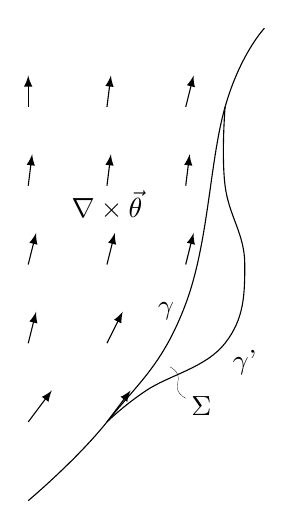
\begin{tikzpicture}

\draw  plot[smooth, tension=.7] coordinates {(0.5,3.5) (0,2.5) (-0.5,0) (-1.5,-1.5) (-2.5,-2.5)};

\node at (-0.75,-0.1) {$\gamma$};


\draw  plot[smooth, tension=.7] coordinates {(0,2.5) (0,1.5) (0.25,0.5) (0,-0.5) (-1,-1.1) (-1.5,-1.5)};

\node at (0.25,-0.75) {$\gamma$'};

\draw[style=ultra thin]  plot[smooth, tension=.7] coordinates {(-0.7,-0.8) (-0.6,-0.9) (-0.6,-1.1) (-0.5,-1.2)};

\node at (-0.3,-1.3) {$\Sigma$};

%\node at (0,0) (Circle) {};
%\draw [<-] (Circle.south)arc(160:-160:-0.2);

\draw [-latex](-0.5,2.5) -- (-0.4,2.9);
\draw [-latex](-1.5,2.5) -- (-1.45,2.9);
\draw [-latex](-2.5,2.5) -- (-2.5,2.9);

\draw [-latex](-0.5,1.5) -- (-0.45,1.9);
\draw [-latex](-1.5,1.5) -- (-1.45,1.9);
\draw [-latex](-2.5,1.5) -- (-2.45,1.9);

\draw [-latex](-0.5,0.5) -- (-0.4,0.9);
\draw [-latex](-1.5,0.5) -- (-1.4,0.9);
\draw [-latex](-2.5,0.5) -- (-2.4,0.9);

\draw [-latex](-1.5,-0.5) -- (-1.3,-0.1);
\draw [-latex](-2.5,-0.5) -- (-2.4,-0.1);

\draw [-latex](-1.5,-1.5) -- (-1.2,-1.1);
\draw [-latex](-2.5,-1.5) -- (-2.2,-1.1);

\node at (-1.5, 1.25) {$\nabla \times \vec{\theta}$};


\end{tikzpicture}
\end{figure}

A way to intuitively understand this is the following. Take a field line $\gamma$ of the curl, a line that is tangent to $\nabla \times \vec{\theta}$ at every point. Between two points, make a small change to it $\gamma'$. Take $\Sigma$ to be a surface enclosed by these lines. The line integral of $\vec{\theta}$ over its contour $\partial \Sigma$ is given by the flow of its curl through $\Sigma$ by the Stokes theorem.

\begin{equation}
\int_{\partial \Sigma} \vec{\theta} \cdot d\vec{\gamma} = \int_{\Sigma} \nabla \times \vec{\theta}  \cdot d\vec{\sigma}
\end{equation}

But remember: $\gamma$ is always tangent to $\nabla \times \vec{\theta}$ by construction. If the variation is small enough, the surface $\Sigma$ is tangent to $\nabla \times \vec{\theta}$ as well. The line integral of $\vec{\theta}$ over the contour $\partial \Sigma$ is zero. This means that the line integral of $\vec{\theta}$ along $\gamma$ is equal to the one along $\gamma'$: small variations of $\gamma$ do not change the line integral.

As $-\vec{\theta}$ is the vector potential for the flow $\vec{S}$, we can write
\begin{equation}
\begin{aligned}
\delta \int \vec{\theta} \cdot d\vec{\gamma} &= \delta \int \vec{\theta} \cdot \vec{S} dt \\
&= \delta \int (\theta^x S^x + \theta ^p S^p + \theta^t S^t)dt \\
&= \delta \int \left( p \frac{dx}{dt} + 0 \frac{dp}{dt} - H \frac{dt}{dt} \right)dt \\
&= \delta \int \left( p \frac{dx}{dt} - H  \right)dt \\
&= \delta \int L dt =  0
\end{aligned}
\label{stationaryAction}
\end{equation}
where $L= \vec{\theta} \cdot \vec{S}$ is the Lagrangian. We recognize the principle of stationary action that gives us the Euler-Lagrange equations. Geometrically, the Lagrangian is the scalar product between the flow and (the opposite of) its vector potential.

\section{Conclusion}

I hope you can appreciate how we have condensed the geometrical description of classical mechanics, which usually takes hundreds of pages to explain, in two pages of simple vector calculus. Once you get used to thinking in these terms, you realize that there are not many moving parts.

This clarifies another important aspect: the conjugate momentum $p$, the Hamiltonian $H$ and the Lagrangian $L$ are all ``unphysical" in the sense that they depend on the choice of the vector potential $-\vec{\theta}$. The vector potential, in fact, is not unique and can be changed without changing the curl. The states and the flow $\vec{S}$, instead, are physical and are uniquely defined by the evolution at hand.

The other interesting part is that the Hamiltonian is the time component of the vector potential. Therefore, under a coordinate transformation, it must change like the time component of a covector. This is one of the features of special relativity and we have already found it without practically doing any work.

The last bit that I want to highlight is that the minimization of the path integral in terms of the Lagrangian is only possible if $p \frac{dx}{dt} - H$ can be expressed in terms of position and velocity. But the minimization in terms of position and momentum is \textbf{always} possible. So the insight that we gathered is more general and it shows how classical mechanics is better understood in the extended phase space.

\end{document}
